\documentclass[addpoints]{exam}
  % Read in shared preamble for all homeworks
  %%%%%%%%%%%%%%%%%%%%%%%%%%%%%%%%%%%%%%%%%%%%%%%%%%%%%%%%%%%%%%%%%%%%
% This is the standard preamble for homework assignments and exams %
%                                                                  %
% -Joshua McNeill (joshua dot mcneill at uga dot edu)              %
%%%%%%%%%%%%%%%%%%%%%%%%%%%%%%%%%%%%%%%%%%%%%%%%%%%%%%%%%%%%%%%%%%%%
% Exam settings
\pointsinmargin
\pointformat{}

% Packages and settings
\usepackage{fontspec}
  \setmainfont{Charis SIL}
\usepackage{tikz}

%% Custom commands
% Instructions for a section
\newcommand{\instr}[1]{
  \begin{center}
    \fbox{
      \parbox{0.85\textwidth}
             {#1}
    }
  \end{center}
}
\newcommand{\lexi}[1]{\textit{#1}}
\newcommand{\gloss}[1]{`#1'}


  % Packages and settings
  \usepackage{graphicx}
    \graphicspath{{../figures/}}

  % Document information
  \title{Homework 1: Phonetics}
  \date{}

\begin{document}
  \maketitle

  % Header
  %%%%%%%%%%%%%%%%%%%%%%%%%%%%%%%%%%%%%%%%%%%%%%%%%%%%%%%%%%%%%%%%%%%%%%%
% This is the the header that all homework assignments and exams use. %
%                                                                     %
% -Joshua McNeill (joshua dot mcneill at uga dot edu)                 %
%%%%%%%%%%%%%%%%%%%%%%%%%%%%%%%%%%%%%%%%%%%%%%%%%%%%%%%%%%%%%%%%%%%%%%%
\noindent\makebox[0.5\textwidth][l]{Name:} \makebox[0.5\textwidth][r]{Course: LING2100, The Study of Language}\\
\makebox[0.5\textwidth][l]{Date:} \makebox[0.5\textwidth][r]{Instructor: Joshua McNeill}


  % Questions
    \instr{Give the IPA transcription of each word that you hear just as it's pronounced. Make sure to include brackets and stress. \emph{The audio can be found on eLC under assignments.} (1 point each)}

  \begin{questions}
      \parbox[t]{0.45\linewidth}{
        \question[1] robust \hrulefill
        \question[1] maid \hrulefill
        \question[1] digress \hrulefill
        \question[1] hub \hrulefill
        \question[1] judge \hrulefill
      }
      \hspace{0.1\linewidth}
      \parbox[t]{0.45\linewidth}{
        \question[1] stutter \hrulefill
        \question[1] linger \hrulefill
        \question[1] tumble \hrulefill
        \question[1] wil \hrulefill
        \question[1] rhythm \hrulefill
      }

    \instr{Give the IPA symbol for the \emph{consonant} that corresponds to the description. Don't forget to include brackets. (1 point each)}
      \parbox[t]{0.45\linewidth}{
        \question[1] Voiceless dental fricative: \hrulefill
        \question[1] Voiced alveolar tap: \hrulefill
        \question[1] Voiceless glottal stop: \hrulefill
        \question[1] Voiceless glottal fricative: \hrulefill
        \question[1] Voiced alveolar approximant: \hrulefill
        \question[1] Voiced alveolar stop: \hrulefill
      }
      \hspace{0.1\linewidth}
      \parbox[t]{0.45\linewidth}{
        \question[1] Voiced labiodental fricative: \hrulefill
        \question[1] Voiced postalveolar fricative: \hrulefill
        \question[1] Voiced velar nasal: \hrulefill
        \question[1] Voiced alveolar fricative: \hrulefill
        \question[1] Voiceless postalveolar fricative: \hrulefill
        \question[1] Voiceless alveolar fricative: \hrulefill
      }

    \instr{Give the IPA symbol for the \emph{vowel} that corresponds to the description. Don't forget to include brackets. (1 point each)}
      \parbox[t]{0.45\linewidth}{
        \question[1] High back rounded: \hrulefill
        \question[1] Near low front unrounded: \hrulefill
        \question[1] High-mid back rounded: \hrulefill
      }
      \hspace{0.1\linewidth}
      \parbox[t]{0.45\linewidth}{
        \question[1] High-mid front unrounded: \hrulefill
        \question[1] Low-mid front unrounded: \hrulefill
        \question[1] Low back unrounded: \hrulefill
      }

    \instr{Give the description -- meaning the voicing, place of articulation, and manner of articulation -- that corresponds to the following \emph{consonant} IPA symbols. (1 point each)}
      \parbox[t]{0.45\linewidth}{
        \question[1] [ʒ]: \hrulefill
        \question[1] [k]: \hrulefill
        \question[1] [n]: \hrulefill
        \question[1] [t]: \hrulefill
        \question[1] [s]: \hrulefill
        \question[1] [l]: \hrulefill
      }
      \hspace{0.1\linewidth}
      \parbox[t]{0.45\linewidth}{
        \question[1] [h]: \hrulefill
        \question[1] [ɾ]: \hrulefill
        \question[1] [ŋ]: \hrulefill
        \question[1] [w]: \hrulefill
        \question[1] [f]: \hrulefill
        \question[1] [dʒ]: \hrulefill
      }

    \instr{Give the description -- meaning the height, advancement, and lip rounding -- that corresponds to the following \emph{vowel} IPA symbols. (1 point each)}
      \parbox[t]{0.45\linewidth}{
        \question[1] [ʊ]: \hrulefill
        \question[1] [ɪ]: \hrulefill
        \question[1] [o]: \hrulefill
      }
      \hspace{0.1\linewidth}
      \parbox[t]{0.45\linewidth}{
        \question[1] [ɔ]: \hrulefill
        \question[1] [u]: \hrulefill
        \question[1] [ɑ]: \hrulefill
      }

    \instr{Give the word, in standard English spelling, that corresponds to the IPA transcription. (1 point each)}
      \parbox[t]{0.45\linewidth}{
        \question[1] [ˈbʌ.səz]: \hrulefill
        \question[1] [θɹ̩ˈmɑ.mɪ.tɹ̩z]: \hrulefill
        \question[1] [əˈfɛk.tɪd]: \hrulefill
        \question[1] [ˈmɛl.tɪŋ]: \hrulefill
        \question[1] [ˈɛ.koʊ]: \hrulefill
        \question[1] [ˈtʃɛɹ]: \hrulefill
        \question[1] [ɹəˈvɔlv]: \hrulefill
        \question[1] [ˈfɹæg.mɛn.tɪd]: \hrulefill
        \question[1] [pɹoʊˌlɪ.fɹ̩ˈeɪ.ʃn̩]: \hrulefill
        \question[1] [ˈspeɪ.ʃəs]: \hrulefill
      }
      \hspace{0.1\linewidth}
      \parbox[t]{0.45\linewidth}{
        \question[1] [ˈtʃɑp.stɪks]: \hrulefill
        \question[1] [kəˈmæn.dɹ̩]: \hrulefill
        \question[1] [ˈtʃeɪs]: \hrulefill
        \question[1] [ˈkɹ̩st]: \hrulefill
        \question[1] [ˈkɹɪ.ɾɪ.saɪzd]: \hrulefill
        \question[1] [pə.blɪˈkeɪ.ʃn̩z]: \hrulefill
        \question[1] [ˈkɑm.plə.mənt]: \hrulefill
        \question[1] [dɪˈʃtɹɪ.bju.ɾɪd]: \hrulefill
        \question[1] [ɪnˈsaɪt]: \hrulefill
        \question[1] [təˈɡɛ.ðɹ̩]: \hrulefill
      }

    \instr{Give the syllable structure, as a tree diagram, for the following one syllable words. (1 point per label)}
      \question[1] [ˈkɹæft]
      \vspace{\stretch{1}}
      \question[1] [ˈɹaɪt]
      \vspace{\stretch{1}}
      \newpage
      \question[1] [ˈhænd]
      \vspace{\stretch{1}}
      \question[1] [ˈlæf]
      \vspace{\stretch{1}}
      \question[1] [ˈɹɛntʃ]
      \vspace{\stretch{1}}
      \question[1] [ˈwɪt]
      \vspace{\stretch{1}}

    \instr{The two spectrograms below represent two different vowels. As best as you can, identify the approximate frequency of F1 and F2 for each. Be aware that three formants are visible. (1 point each)}
      \question[1]
        \begin{minipage}{0.45\linewidth}
          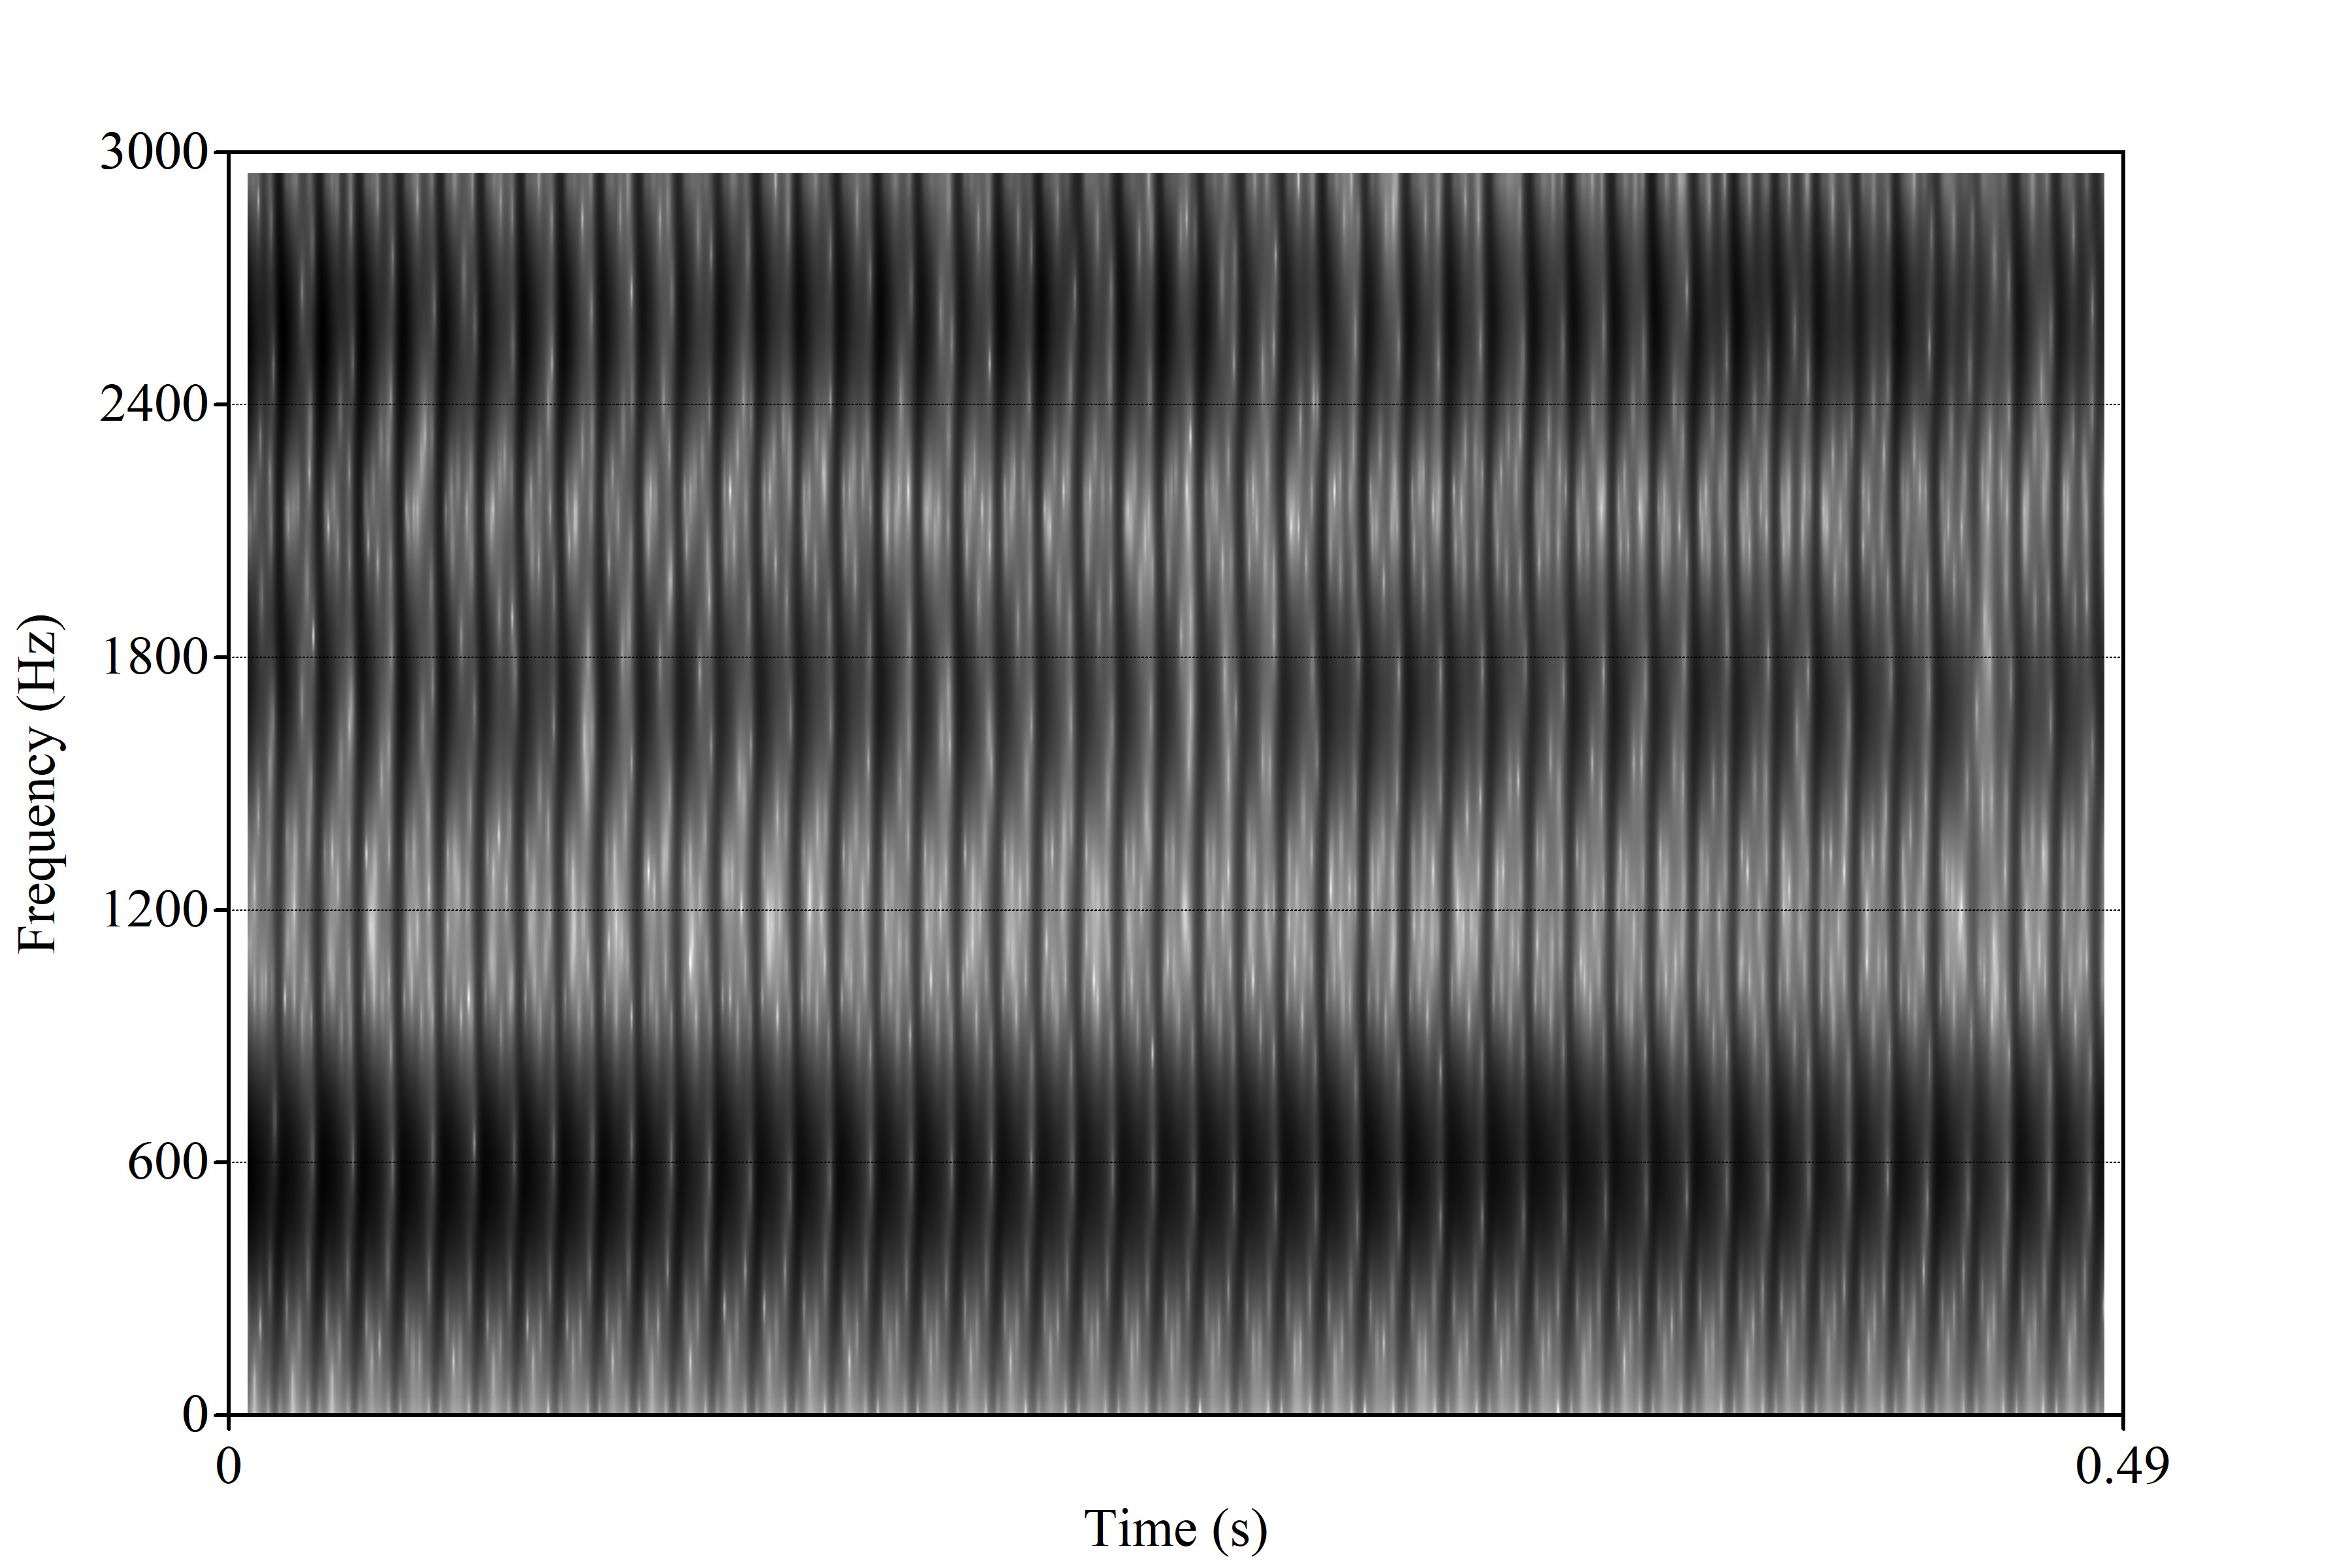
\includegraphics[scale=0.6]{vowel4.jpg}
        \end{minipage}\hspace{0.1\linewidth}
        \begin{minipage}{0.45\linewidth}
          \begin{itemize}
            \item[F1:] \hrulefill
            \item[F2:] \hrulefill
          \end{itemize}
        \end{minipage}

      \newpage
      \question[1]
        \begin{minipage}{0.45\linewidth}
          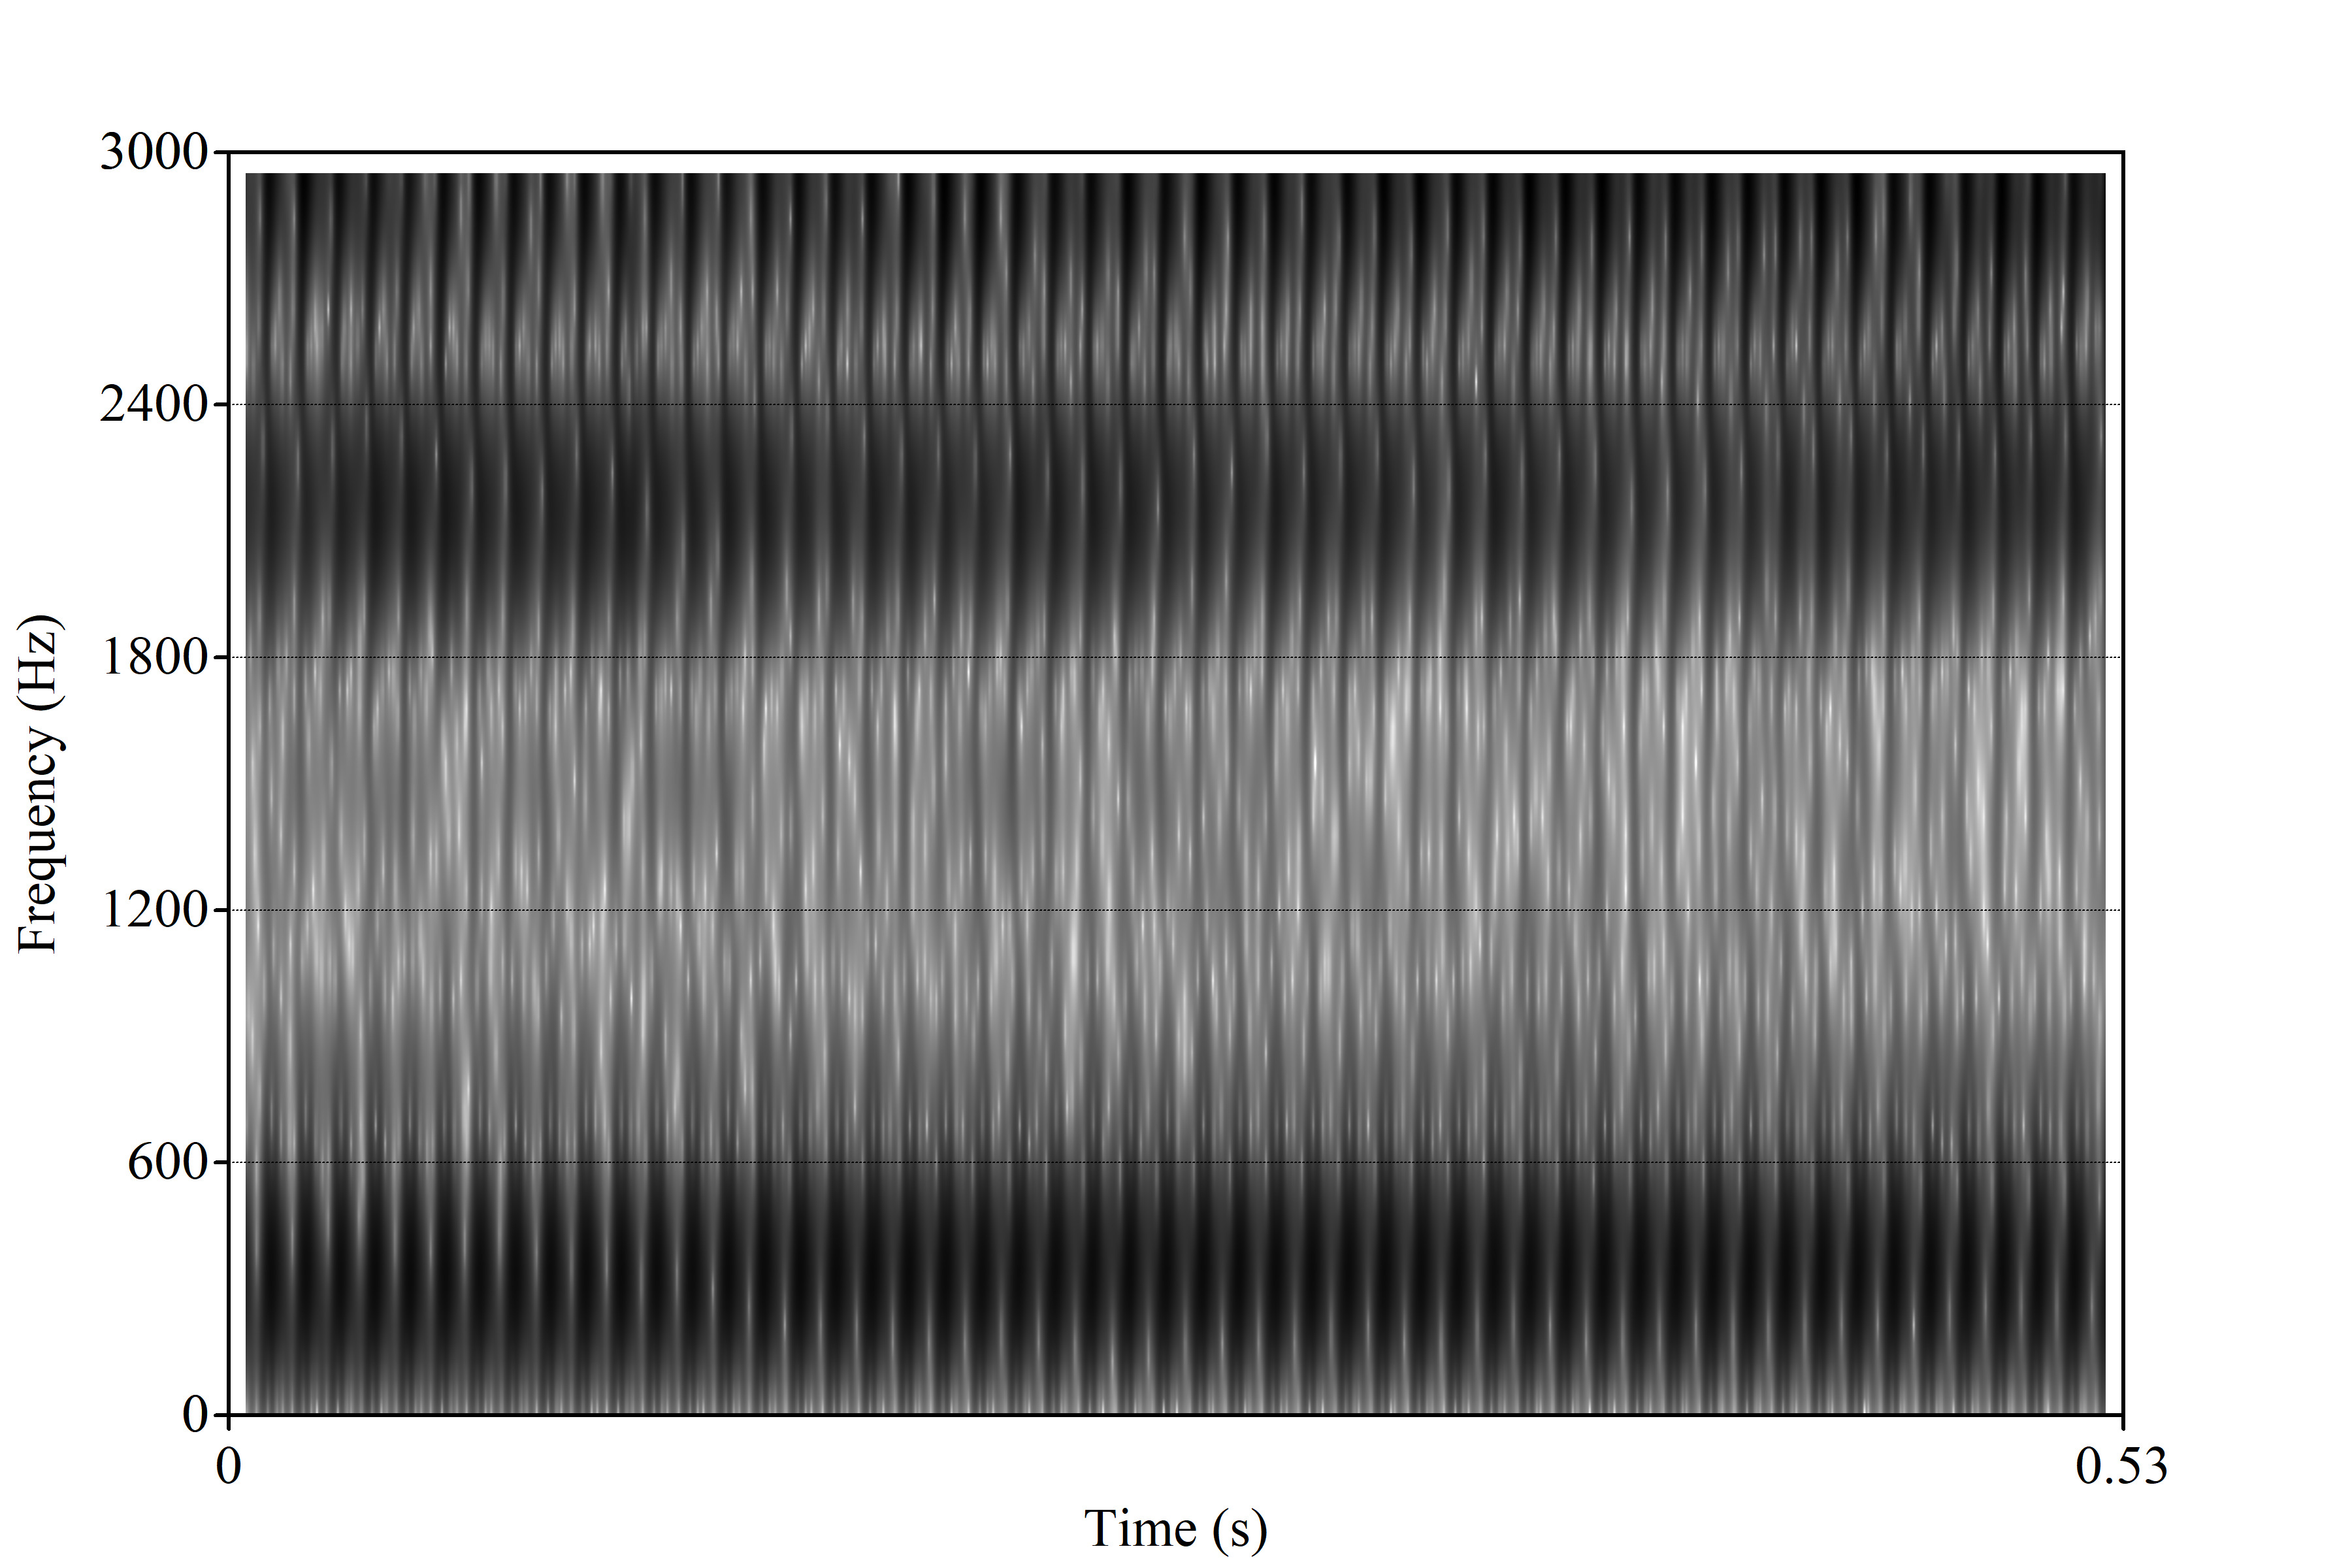
\includegraphics[scale=0.6]{vowel2.jpg}
        \end{minipage}\hspace{0.1\linewidth}
        \begin{minipage}{0.45\linewidth}
          \begin{itemize}
            \item[F1:] \hrulefill
            \item[F2:] \hrulefill
          \end{itemize}
        \end{minipage}
      \question[1]
        \begin{minipage}{0.45\linewidth}
          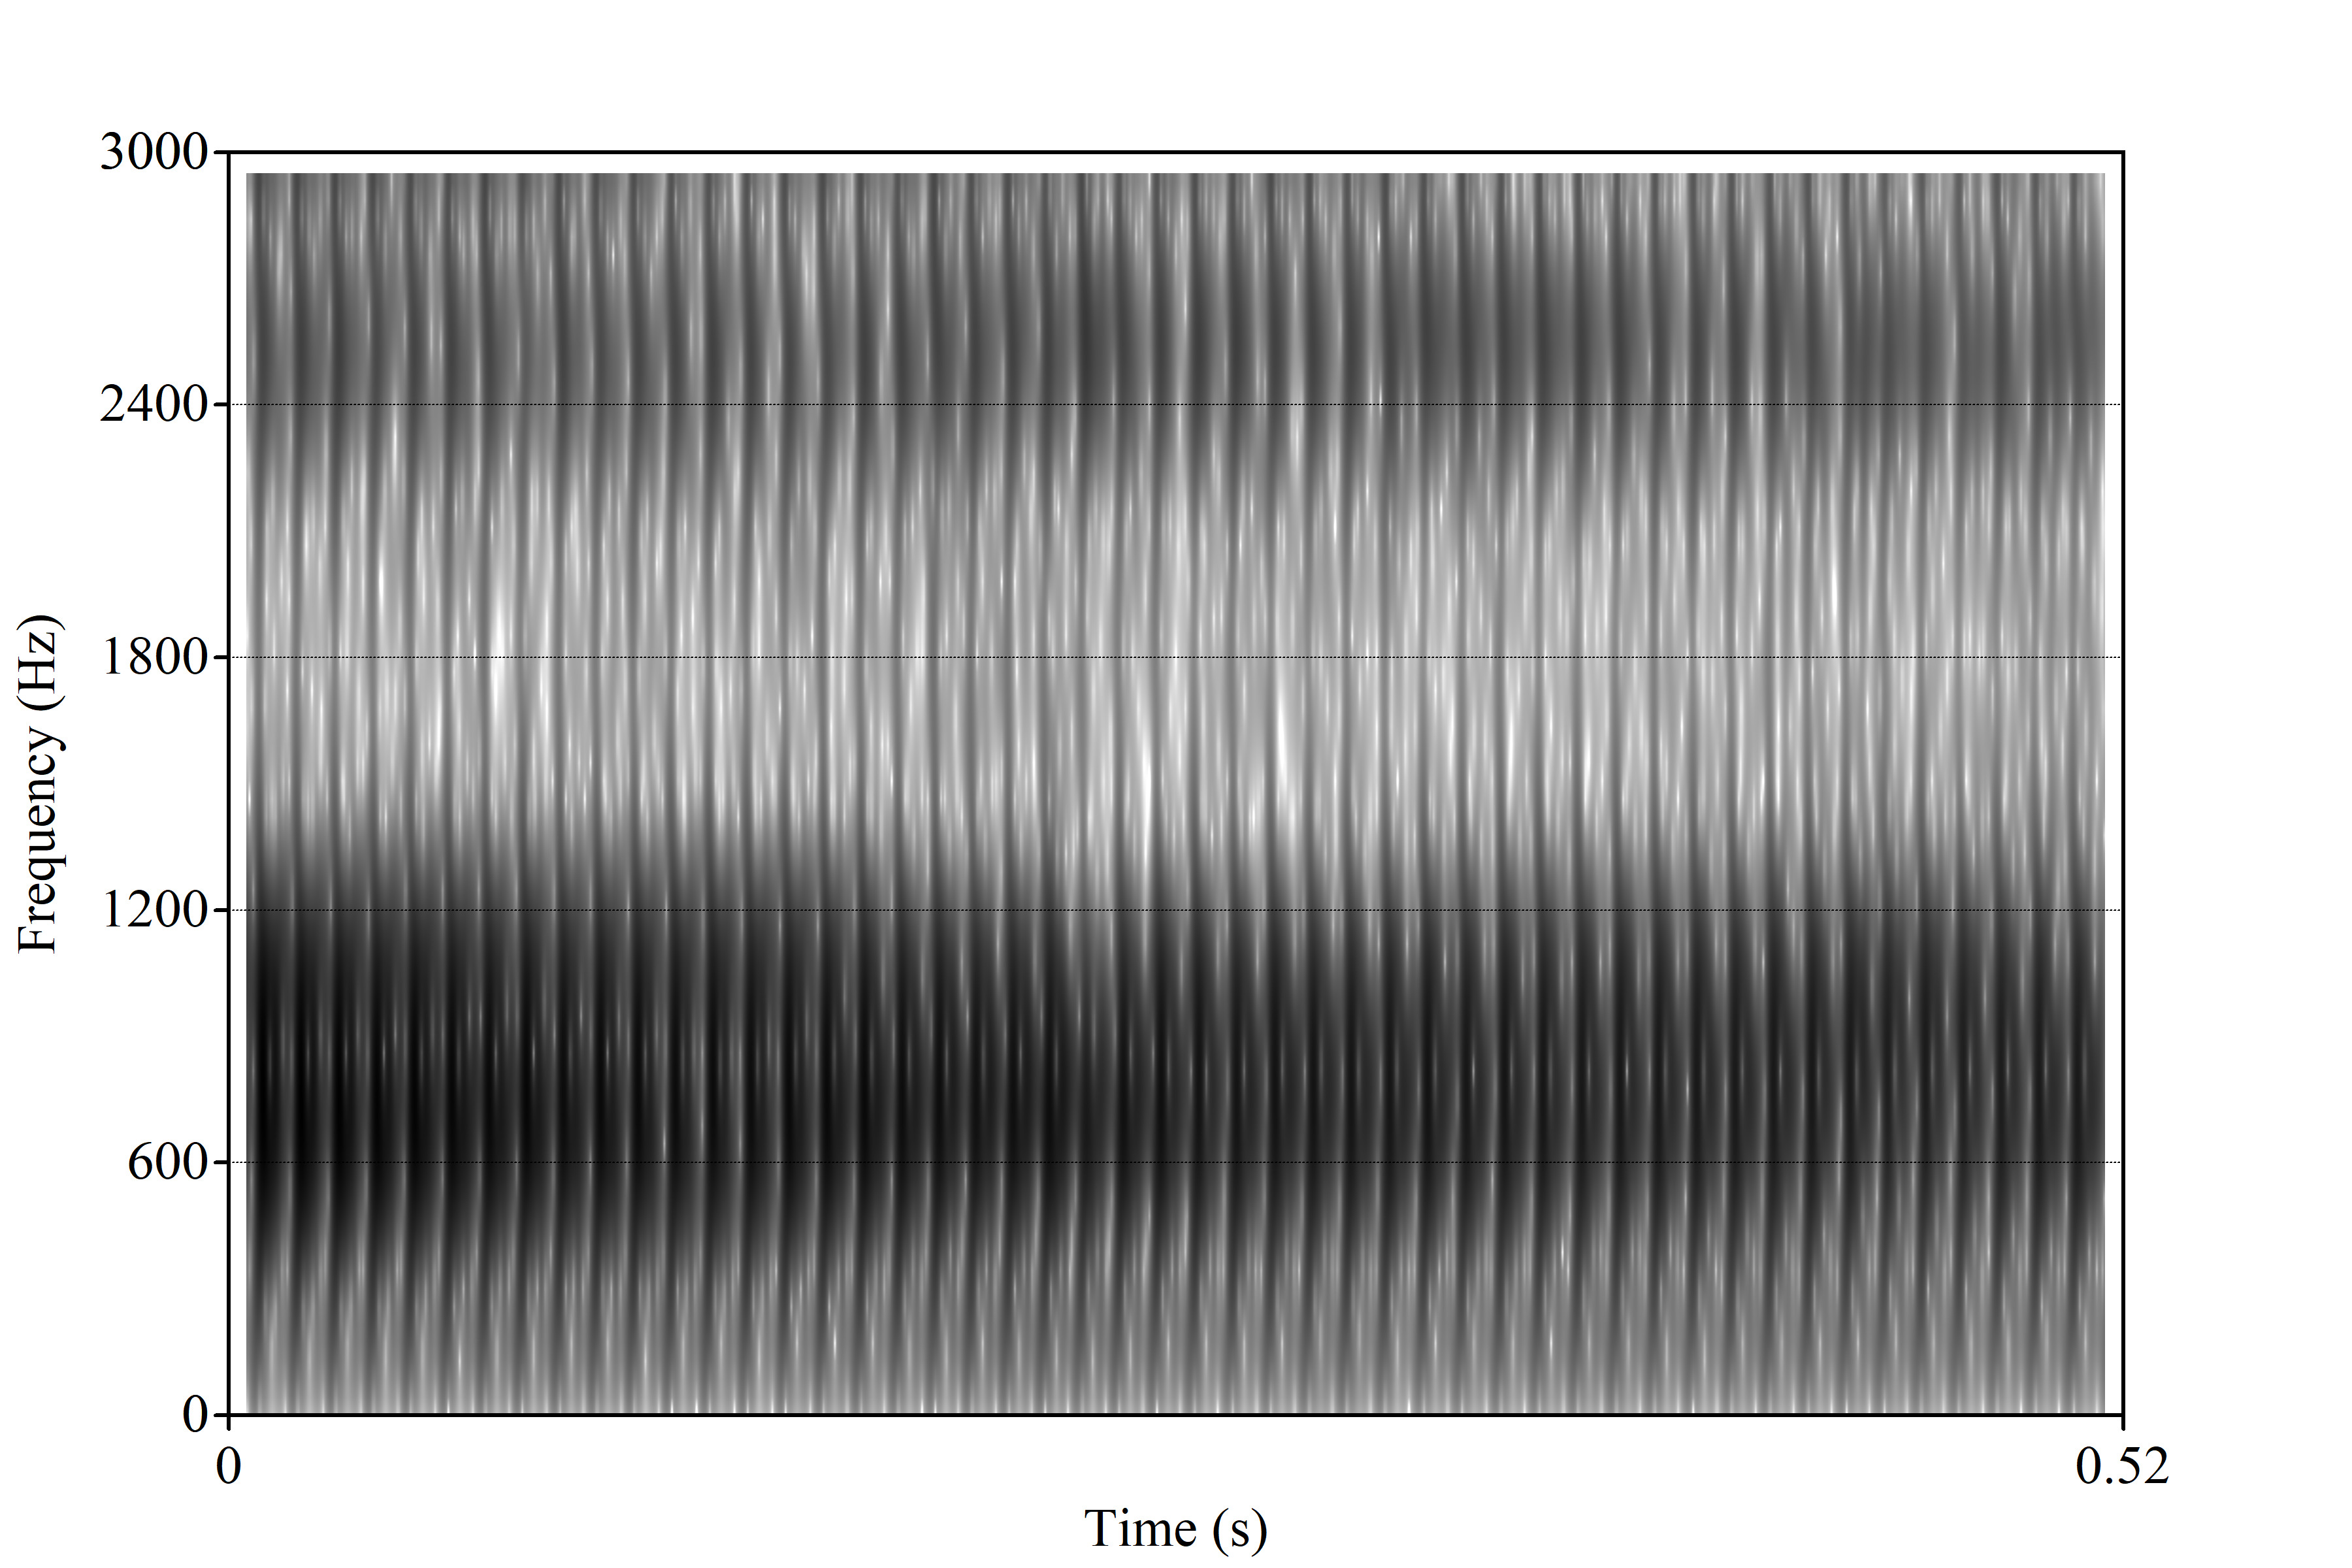
\includegraphics[scale=0.6]{vowel6.jpg}
        \end{minipage}\hspace{0.1\linewidth}
        \begin{minipage}{0.45\linewidth}
          \begin{itemize}
            \item[F1:] \hrulefill
            \item[F2:] \hrulefill
          \end{itemize}
        \end{minipage}
  \end{questions}

  \vspace{1.25cm}

  % Grade
  \begin{center}
    \gradetable[v][pages]
  \end{center}
\end{document}
